\documentclass[10pt,a4paper]{article}
\usepackage[margin=2.1cm]{geometry}
\usepackage{amsmath,amssymb,bm,physics}
\usepackage{graphicx,booktabs,xcolor,enumitem,hyperref}
\hypersetup{colorlinks,linkcolor=blue!50!black,urlcolor=blue!50!black}
\newcommand{\kb}{\bar\kappa}
\newcommand{\ka}{\kappa_1}
\newcommand{\kc}{\kappa_2}
\newcommand{\note}[1]{\par\smallskip\noindent\colorbox{gray!12}{\parbox{\dimexpr\linewidth-2\fboxsep}{\small #1}}\par\smallskip}
\newcommand{\evd}[1]{\textsf{\small[#1]}}
\title{TOP-Q --- Day 1 worked notes\\[2pt]\large Coupled-mode theory $\to$ SSH Hamiltonian $\to$ Bloch bands $\to$ validated code}
\author{PH 5110 term paper --- Kotapati Kishore (EE26E016)}
\date{22 October 2026}
\begin{document}\maketitle

\note{\textbf{How to use these notes.} This is a fully worked reference. It is only useful if you can reproduce it:
close the PDF and re-derive Sections~1 and~2 on paper, then explain each test in Section~3 aloud.
Evidence labels used throughout: \evd{Derived} analytic result; \evd{Assumption}; \evd{Verified-by-test};
\evd{Simulated} numerical observation; \evd{Literature}; \evd{Hypothesis}.}

\tableofcontents

%=====================================================================
\section{Block 1 --- Deriving the coupled-mode equations}
%=====================================================================
\subsection{Physical picture}
A single-mode dielectric waveguide confines light in its core, but the mode field does not stop at the
core boundary: it decays \emph{evanescently} into the cladding. Place a second identical waveguide a
gap $g$ away and the tail of mode~1 overlaps core~2. That overlap acts as a weak, distributed source for
mode~2, so power transfers back and forth along $z$. Coupled-mode theory (CMT) keeps the
\emph{shape} of each isolated mode and lets only its complex amplitude $a_n(z)$ evolve.

\subsection{Assumptions \evd{Assumption}}
\begin{enumerate}[label=A\arabic*,itemsep=1pt]
\item Monochromatic field, angular frequency $\omega$, time dependence $e^{-i\omega t}$; forward propagation $e^{+i\beta z}$.
\item Scalar, paraxial, weakly guiding: one polarisation, so $E(x,y,z)$ obeys the scalar Helmholtz equation.
\item Identical single-mode waveguides: all isolated modes have the same $\beta_0$ and shape (translated).
\item Weak coupling: $\kappa\ll\beta_0$; modal overlaps $\int e_ne_m\,dA$ ($n\neq m$) negligible.
\item Lossless dielectrics (real index): this makes $H$ Hermitian. Loss is added deliberately on Day 5.
\item $z$-invariant structure (straight parallel guides): $\kappa$ independent of $z$.
\end{enumerate}

\subsection{Step 1: wave equation}
For a weakly guiding medium the transverse field obeys
\begin{equation}
\nabla^2E+k_0^2n^2(x,y)\,E=0,\qquad k_0=\frac{2\pi}{\lambda}=\frac{\omega}{c}\ \ [\mathrm{m^{-1}}].\label{eq:helm}
\end{equation}
$n^2(x,y)$ is the relative permittivity profile of the whole array.

\subsection{Step 2: isolated waveguide $m$}
Let $n_m^2(x,y)$ be the profile of cladding plus \emph{only} core $m$. Its guided mode $e_m(x,y)e^{i\beta_0 z}$ satisfies
\begin{equation}
\nabla_t^2e_m+\big(k_0^2n_m^2-\beta_0^2\big)e_m=0,\qquad \nabla_t^2=\partial_x^2+\partial_y^2 .\label{eq:mode}
\end{equation}
$e_m$ is real and positive everywhere for a fundamental mode (no nodes) --- this matters for the sign of $\kappa$.

\subsection{Step 3: the array seen from waveguide $m$}
Write the full profile as $n^2=n_m^2+\sum_{p\neq m}\Delta n_p^2$, where $\Delta n_p^2(x,y)=n_{\rm core}^2-n_{\rm cl}^2$ inside core $p$ and $0$ elsewhere.

\subsection{Step 4(a): substitute the ansatz}
Ansatz: $E=\sum_m a_m(z)\,e_m(x,y)\,e^{i\beta_0z}$. Using $\partial_z^2(a e^{i\beta_0z})=(a''+2i\beta_0a'-\beta_0^2a)e^{i\beta_0z}$:
\begin{align*}
\nabla^2E&=\textstyle\sum_m e^{i\beta_0z}\big[a_m\nabla_t^2e_m+e_m(a_m''+2i\beta_0a_m'-\beta_0^2a_m)\big],\\
k_0^2n^2E&=\textstyle\sum_m e^{i\beta_0z}\,k_0^2\big(n_m^2+\sum_{p\neq m}\Delta n_p^2\big)a_me_m .
\end{align*}
Add them and replace $\nabla_t^2e_m$ using \eqref{eq:mode}: the terms $-(k_0^2n_m^2-\beta_0^2)a_me_m$, $-\beta_0^2a_me_m$ and $+k_0^2n_m^2a_me_m$ cancel exactly. What survives is \evd{Derived}
\begin{equation}
\sum_m\Big[(a_m''+2i\beta_0a_m')\,e_m+k_0^2\,a_m\sum_{p\neq m}\Delta n_p^2\,e_m\Big]=0. \label{eq:4a}
\end{equation}
\emph{Interpretation:} the isolated-mode physics cancels; only the ``extra'' index of the \emph{other} cores drives changes in $a_m$.

\subsection{Step 4(b): slowly varying envelope approximation (SVEA)}
Coupling makes $a_m$ vary on the length scale $1/\kappa$, so $a_m'\sim\kappa a_m$ and $a_m''\sim\kappa^2a_m$. Then
\[
\frac{|a_m''|}{2\beta_0|a_m'|}\sim\frac{\kappa}{2\beta_0}\ll1\quad\text{by A4,}
\]
so $a_m''$ is dropped. Physically: the envelope changes negligibly over one optical wavelength in the medium. \evd{Assumption}

\subsection{Step 4(c): project onto mode $n$}
Multiply \eqref{eq:4a} (without $a''$) by $e_n$ and integrate over the cross-section. By A4, $\int e_me_n\,dA\approx\delta_{mn}\int e_n^2\,dA$:
\[
2i\beta_0\,a_n'\int e_n^2\,dA=-k_0^2\sum_m a_m\int\Big(\sum_{p\neq m}\Delta n_p^2\Big)e_me_n\,dA .
\]
Divide by $2i\beta_0\int e_n^2dA$ and use $-1/i=+i$: \evd{Derived}
\begin{equation}
\boxed{\ \frac{da_n}{dz}=i\sum_m\kappa_{nm}a_m,\qquad
\kappa_{nm}=\frac{k_0^2}{2\beta_0}\,\frac{\int\big(\sum_{p\neq m}\Delta n_p^2\big)e_m e_n\,dA}{\int e_n^2\,dA}\ }\label{eq:cmt}
\end{equation}
\textbf{Nearest neighbours} ($m=n\pm1$): the integrand needs $e_n$ to be large, i.e.\ we are inside core $n$, so the dominant term of $\sum_{p\neq m}$ is $p=n$:
\begin{equation}
\kappa_{n,n\pm1}\simeq\frac{k_0^2}{2\beta_0}\,\frac{\int_{\text{core }n}\Delta n_n^2\,e_n\,e_{n\pm1}\,dA}{\int e_n^2\,dA}. \label{eq:kappa}
\end{equation}
Non-nearest neighbours involve $e_{n\pm2}$ inside core $n$, which is exponentially smaller (Section~1.10) --- this is the nearest-neighbour approximation \evd{Assumption}.

\subsection{Matrix form and power conservation}
Collect amplitudes in $\bm a=(a_1,\dots,a_M)^T$: $\;d\bm a/dz=iH\bm a$, $H_{nm}=\kappa_{nm}$ (off-diagonal) and $H_{nn}=\delta\beta_n$ (on-site detuning + self-shift). Then
\[
\frac{d}{dz}\,\bm a^\dagger\bm a=\bm a^\dagger\big(-iH^\dagger+iH\big)\bm a=0\quad\text{iff }H=H^\dagger .
\]
So lossless $\Leftrightarrow$ Hermitian $H$ $\Leftrightarrow$ $\sum_n|a_n|^2$ conserved \evd{Derived}. (For $|a_n|^2$ to \emph{be} power in watts, $e_n$ must be normalised so that $\frac{\beta_0}{2\omega\mu_0}\int e_n^2dA=1$; the dynamics do not depend on this choice.)
Solution: $\bm a(z)=e^{iHz}\bm a(0)$. If $H\bm\psi=b\bm\psi$, then a launched supermode evolves as $\bm\psi e^{ibz}$, i.e.\ total phase $e^{i(\beta_0+b)z}$: \textbf{eigenvalue $b$ = propagation-constant shift.}

\subsection{Answers to the Block-1 questions}
\textbf{Q1 (units).} $[k_0^2]=\mathrm{m^{-2}}$, $[\beta_0]=\mathrm{m^{-1}}$, $\Delta n^2$ dimensionless, and the ratio of integrals is dimensionless (same $e^2\,dA$ in numerator and denominator). So $[\kappa]=\mathrm{m^{-2}}/\mathrm{m^{-1}}=\mathrm{m^{-1}}$ (rad/m). $\checkmark$

\textbf{Q2 (sign).} Inside core $n$: $\Delta n_n^2>0$ (core index exceeds cladding), $e_n>0$, $e_{n\pm1}>0$ (fundamental modes have no nodes). The integrand is positive, so $\kappa>0$. With the opposite convention $e^{-i\beta z}$, step~4(c) gives $da/dz=-iHa$ with the same positive $\kappa$; equivalently $H\to-H$, so $b\to-b$. Because the SSH spectrum is symmetric about zero (Section~2.6) the band \emph{shapes} are unchanged, but the meaning of ``$b>0$'' (faster vs.\ slower phase) flips. Always state your convention --- that is why it is fixed in the conventions sheet.

\textbf{Q3 (self-shift).} The $m=n$ term of \eqref{eq:cmt} gives $\sigma_n=\frac{k_0^2}{2\beta_0}\int\sum_{p\neq n}\Delta n_p^2e_n^2\,dA/\int e_n^2dA$: the neighbours' cores sit in mode $n$'s own tail. Every \emph{interior} guide has two neighbours, so the same $\sigma$; we absorb it into $\beta_0$. The \textbf{two end guides have only one neighbour}, so their self-shift is $\approx\sigma/2$ smaller: an \emph{on-site detuning localised exactly where the edge mode lives}. Because $\sigma\propto(e^{-\gamma g})^2$ while $\kappa\propto e^{-\gamma g}$, it is second order, $\sigma/\kappa\sim e^{-\gamma g}\ll1$, but it is a genuine chiral-symmetry-breaking term in a real device. \textbf{Record as Limitation L1.}

\textbf{Q4 (exponential gap dependence).} Outside its core, mode $m$ satisfies $\nabla_t^2e_m=(\beta_0^2-k_0^2n_{\rm cl}^2)e_m\equiv\gamma^2e_m$, so it decays as $e^{-\gamma r}$ (slab: exactly $e^{-\gamma|x|}$; 2-D: $K_0(\gamma r)\sim e^{-\gamma r}/\sqrt r$). Inside core $n$, a distance $\approx g$ from the edge of core $m$, $e_m\propto e^{-\gamma g}$, hence
\[
\kappa(g)\approx\kappa_0e^{-\gamma g}=\kappa_0e^{-g/g_0},\qquad g_0=\gamma^{-1},\qquad \frac{\delta\kappa}{\kappa}=-\gamma\,\delta g .
\]
A fixed gap error $\delta g$ therefore produces a fixed \emph{fractional} coupling error. That is the physical justification for \textbf{multiplicative} coupling disorder $\kappa\to\kappa(1+\epsilon)$ (Day 3) \evd{Derived}.

%=====================================================================
\section{Block 3 --- SSH equations, Bloch Hamiltonian, bands}
%=====================================================================
\subsection{Real-space SSH equations}
Alternate the gaps $g_1,g_2,g_1,\dots$ so the couplings alternate $\ka,\kc$. Group guides in unit cells $n=1,\dots,N$, each with an A and a B guide; $\ka$ couples $A_n\!\leftrightarrow\!B_n$ (intra-cell), $\kc$ couples $B_n\!\leftrightarrow\!A_{n+1}$ (inter-cell). With $\delta\beta_n=0$ (identical guides), \eqref{eq:cmt} gives \evd{Derived}
\begin{equation}
\frac{da_n}{dz}=i(\ka b_n+\kc b_{n-1}),\qquad \frac{db_n}{dz}=i(\ka a_n+\kc a_{n+1}). \label{eq:ssh}
\end{equation}
Key structure: A couples only to B, B only to A (\emph{bipartite} lattice). Real-space $H$ for $M=6$:
\[
H=\begin{pmatrix}0&\ka&&&&\\ \ka&0&\kc&&&\\ &\kc&0&\ka&&\\ &&\ka&0&\kc&\\ &&&\kc&0&\ka\\ &&&&\ka&0\end{pmatrix}.
\]

\subsection{Bloch's theorem on a lattice}
In an infinite (or periodic) array, $H$ commutes with the one-cell translation $T:(a_n,b_n)\mapsto(a_{n+1},b_{n+1})$. Commuting operators share eigenvectors, and $T$ is unitary, so its eigenvalues are $e^{ik}$. Hence eigenmodes take the form $a_n=a\,e^{ikn}$, $b_n=b\,e^{ikn}$, with $k=q\Lambda$ dimensionless ($\Lambda$ = transverse cell period = centre-to-centre distance over two guides) and $k\in(-\pi,\pi]$ (the Brillouin zone; $k$ and $k+2\pi$ are the same state).

\subsection{Bloch Hamiltonian}
Substitute into \eqref{eq:ssh}: $b_{n-1}=b\,e^{ik(n-1)}$, $a_{n+1}=a\,e^{ik(n+1)}$; cancel $e^{ikn}$:
\[
\frac{d}{dz}\begin{pmatrix}a\\b\end{pmatrix}=i\,H(k)\begin{pmatrix}a\\b\end{pmatrix},\qquad
\boxed{H(k)=\begin{pmatrix}0&h(k)\\h^*(k)&0\end{pmatrix},\quad h(k)=\ka+\kc e^{-ik}} \evd{Derived}
\]

\subsection{Bands}
$\det(H(k)-b\mathbb 1)=b^2-|h|^2=0$, and $|h|^2=(\ka+\kc\cos k)^2+\kc^2\sin^2k=\ka^2+\kc^2+2\ka\kc\cos k$:
\begin{equation}
\boxed{b_\pm(k)=\pm\sqrt{\ka^2+\kc^2+2\ka\kc\cos k}} \evd{Derived}\label{eq:bands}
\end{equation}
\begin{itemize}[itemsep=1pt]
\item Maximum of $|b|$ at $k=0$: $\ka+\kc$ (total band extent $2(\ka+\kc)$).
\item Minimum at $k=\pi$: $|\ka-\kc|$. \textbf{Gap} $=2|\ka-\kc|$, centred on $b=0$, i.e.\ on $\beta_0$.
\item Gap closes only for $\ka=\kc$ (uniform array; folded band $b=\pm2\kappa\cos(k/2)$).
\item Physical meaning of the slope: $\partial b/\partial k$ is the transverse group velocity (how fast light walks sideways per unit $z$, in cells); its spread is \emph{discrete diffraction}.
\end{itemize}

\subsection{\texorpdfstring{$\bm d$-vector form and what a $\sigma_z$ term would mean}{d-vector form and what a sigma-z term would mean}}
Any $2\times2$ Hermitian matrix is $d_0\mathbb 1+\bm d\cdot\bm\sigma$. Matching $h=d_x-id_y$:
\[
d_x(k)=\ka+\kc\cos k,\qquad d_y(k)=\kc\sin k,\qquad d_z=d_0=0,\qquad b_\pm=\pm|\bm d| .
\]
\begin{itemize}[itemsep=1pt]
\item $d_z\sigma_z$ = \textbf{opposite} detunings on A and B: $\delta\beta_A=+d_z$, $\delta\beta_B=-d_z$ (alternating guide widths) --- the Rice--Mele model. It opens a gap even at $\ka=\kc$ and moves states off $b=0$.
\item $d_0\mathbb 1$ = a \textbf{common} shift of every guide's $\beta$ (e.g.\ a uniform width error): shifts all $b$ by $d_0$.
\item With $d_z=d_0=0$: $\sigma_zH(k)\sigma_z=-H(k)$. This is \textbf{chiral (sublattice) symmetry}; it forces eigenvalues in $\pm b$ pairs. Both perturbations above break it. (Developed on Day 2.)
\end{itemize}

\subsection{\texorpdfstring{Why $\pm\delta$ give identical bulk bands}{Why +-delta give identical bulk bands}}
Parametrise $\ka=\kb(1-\delta)$, $\kc=\kb(1+\delta)$. Equation \eqref{eq:bands} is symmetric under $\ka\leftrightarrow\kc$ ($\delta\to-\delta$). So \textbf{the bulk spectrum cannot distinguish the two dimerisations}. They differ only in how the chain is \emph{cut}: an A-terminated chain ends on a weak bond if $\ka<\kc$ (``dangling'' end guide) and on a strong bond if $\ka>\kc$. Fig.~\ref{fig:bands}(b) shows the consequence.

\note{\textbf{Correction to my earlier instructions.} On 21 Oct I wrote that the bands for $\ka/\kc=0.5$ and $2$, plotted in units of $\kc$, are identical. That is wrong as stated: in units of $\kc$ the second case is the first scaled by~2. They are identical when the \emph{mean} coupling $\kb$ is held fixed (equivalently, under $\ka\leftrightarrow\kc$). The figure below uses this fixed-$\kb$ parametrisation.}

\subsection{Finite rings: which $k$ are allowed}
A ring of $N$ cells requires $a_{n+N}=a_n\Rightarrow e^{ikN}=1\Rightarrow k_m=2\pi m/N$, $m=0,\dots,N-1$. Its $2N$ eigenvalues are exactly $b_\pm(k_m)$ --- no approximation. This is what makes the ring a sharp numerical test of \eqref{eq:bands}. If $N$ is even, $k=\pi$ is allowed, so the ring gap equals $2|\ka-\kc|$ exactly.

%=====================================================================
\section{Block 4 --- Implementation and validation}
%=====================================================================
\subsection{Module design (\texttt{topq/ssh.py})}
\begin{tabular}{@{}p{0.33\linewidth}p{0.62\linewidth}@{}}\toprule
Function & Purpose / design decision\\\midrule
\texttt{ssh\_couplings(M,k1,k2)} & $[\ka,\kc,\ka,\dots]$, length $M-1$; chain always starts on A with $\ka$ (conventions sheet).\\
\texttt{hamiltonian\_from\_couplings} & General tridiagonal builder from an arbitrary coupling array + optional on-site array + optional ring closure. Day 3 disorder will pass perturbed arrays here, so disorder and clean code share one builder.\\
\texttt{ssh\_hamiltonian(M,k1,k2,...)} & Thin wrapper; ring requires even $M$ (otherwise the closure would join A to A and break the cell structure).\\
\texttt{bloch\_hamiltonian(k,...)} & Vectorised $2\times2$ $H(k)$, shape \texttt{k.shape+(2,2)}.\\
\texttt{bloch\_bands(k,...)} & Eq.~\eqref{eq:bands}; \texttt{clip} protects $\sqrt{\cdot}$ from $-10^{-17}$ round-off at $\ka=\kc,k=\pi$.\\\bottomrule
\end{tabular}

\textbf{Why \texttt{eigh}, not \texttt{eig}:} for Hermitian matrices \texttt{numpy.linalg.eigh} uses a symmetric solver: real sorted eigenvalues, orthonormal eigenvectors, backward-stable. \texttt{eig} may return tiny spurious imaginary parts and non-orthogonal vectors for degenerate eigenvalues. (Once loss is added on Day 5 $H$ is non-Hermitian and we must switch to \texttt{eig} deliberately.)

\textbf{Units:} the code is unit-agnostic. Whatever unit you pass $\ka,\kc$ in (e.g.\ mm$^{-1}$), $b$ comes out in the same unit.

\subsection{Test suite (\texttt{tests/test\_ssh.py}) --- 23 tests, all pass \evd{Verified-by-test}}
\begin{tabular}{@{}p{0.27\linewidth}p{0.68\linewidth}@{}}\toprule
Test & What it proves (and why it is independent)\\\midrule
Ring vs.\ analytic & Real-space ring eigenvalues equal \eqref{eq:bands} at $k_m$ to $<10^{-12}$ for 4 coupling pairs. Independent: real-space matrix vs.\ Bloch algebra.\\
Real symmetric & Lossless $H$ is Hermitian (Section~1.9).\\
Spectrum symmetric & Open chains ($M=40,41$) have $\{b\}=\{-b\}$: numerical signature of chiral symmetry.\\
Ring gap & Gap $=2|\ka-\kc|$ (even $N$ contains $k=\pi$).\\
Bad inputs & Negative coupling, odd ring, wrong on-site length, NaN all raise \texttt{ValueError}.\\
Bloch consistency & $H(k)$ Hermitian, $2\pi$-periodic, \texttt{eigvalsh}$(H(k))=b_\pm(k)$.\\
Uniform open chain & $\ka=\kc$: $b_j=2\kappa\cos\frac{\pi j}{M+1}$ --- a textbook result derived without Bloch theory.\\
Fully dimerised & $\kc=0$: isolated dimers $\pm\ka$. $\ka=0$: dimers $\pm\kc$ \emph{plus two isolated end guides at exactly $b=0$} --- the extreme limit of the edge states.\\\bottomrule
\end{tabular}

\textbf{Do the tests have teeth? (mutation test).} I deliberately injected three bugs and re-ran the suite: closing the ring with $\ka$ instead of $\kc$ (6 failures), $\cos k\to\sin k$ in the bands (5 failures), all couplings set to $\ka$ (5 failures). A test suite that cannot fail is not evidence; this one catches realistic mistakes.

\subsection{Independent momentum assignment for the figure}
Plotting ring eigenvalues at the analytic $k_m$ would be circular. Instead, for each real eigenvector $\bm\psi$ of the ring, compute $\langle\bm\psi|T|\bm\psi\rangle$ with $T$ = shift by two sites. A real eigenvector is an equal mixture of $\pm k$ Bloch states, so $\langle T\rangle=\tfrac12(e^{ik}+e^{-ik})=\cos k$, giving $|k|=\arccos\langle T\rangle$ \emph{from the eigenvector alone}. Point-wise agreement with \eqref{eq:bands}: $\le2\times10^{-15}$ for $\delta=\pm1/3$. For $\delta=0$ it is $3\times10^{-8}$: not a bug, but the ill-conditioning of $\arccos$ near $\pm1$ ($\delta k\sim\sqrt{\epsilon}$ for round-off $\epsilon\sim10^{-16}$) plus the band touching at $k=\pi$. \evd{Simulated}

%=====================================================================
\section{Block 5 --- Figure, observations, reading}
%=====================================================================
\begin{figure}[h]\centering
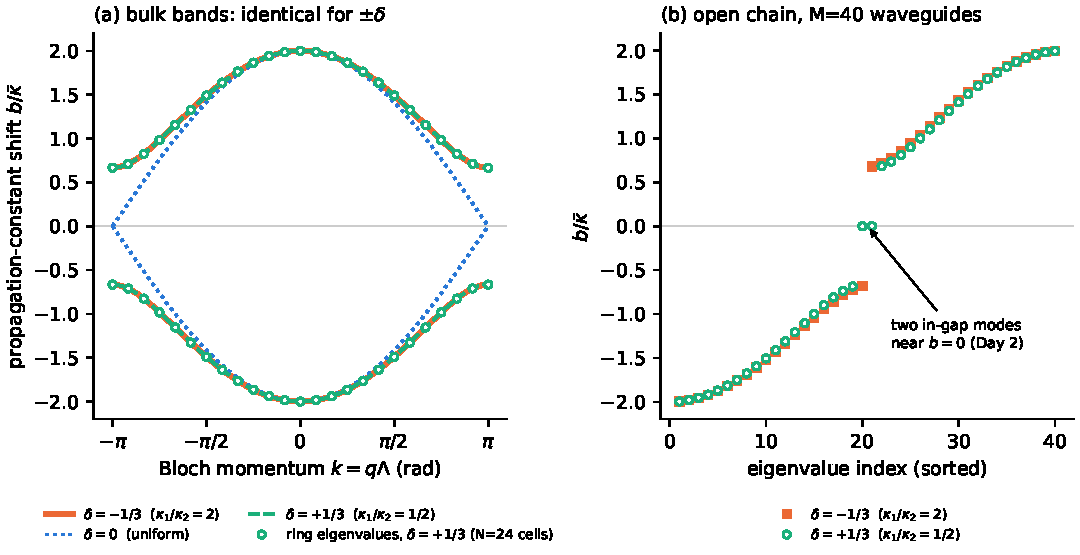
\includegraphics[width=\linewidth]{../../figures/fig_bands.pdf}
\caption{(a) Bulk bands \eqref{eq:bands} for $\delta=-1/3,0,+1/3$ at fixed $\kb$; circles: real-space ring eigenvalues ($N=24$ cells, $\delta=+1/3$) with momenta assigned from eigenvectors. (b) Spectrum of an open chain of $M=40$ guides for $\delta=\pm1/3$. Generated by \texttt{scripts/day1\_bands.py} from \texttt{data/day1\_bands.npz}; deterministic, no random numbers.}
\label{fig:bands}
\end{figure}

\textbf{Observations} \evd{Simulated}
\begin{enumerate}[itemsep=1pt]
\item The $\delta=\pm1/3$ bulk bands coincide; ring eigenvalues lie on them to $10^{-15}$.
\item Gap: $2|\ka-\kc|/\kb=4/3$; band edges at $\pm2/3$ and $\pm2$ (in units of $\kb$), as predicted.
\item Open chain: $\delta=+1/3$ ($\ka<\kc$) has \textbf{two} eigenvalues inside the gap at $|b|/\kb=9.54\times10^{-7}$; $\delta=-1/3$ has none (smallest $|b|/\kb=0.680$, just above the bulk edge $2/3$ because of finite size).
\item The two in-gap values are not exactly 0: they are $\pm$-split. Their magnitude equals $(\ka/\kc)^{N}=(1/2)^{20}=9.537\times10^{-7}$ to the digits shown --- a strong hint of exponential hybridisation of the two edge modes. \evd{Hypothesis --- to be derived on Day 2, not yet claimed.}
\end{enumerate}

\subsection{Reading notes: Su, Schrieffer \& Heeger}
\textbf{Citation.} W.~P.~Su, J.~R.~Schrieffer, A.~J.~Heeger, ``Solitons in Polyacetylene,'' \emph{Phys.\ Rev.\ Lett.}\ \textbf{42}, 1698 (1979), doi:10.1103/PhysRevLett.42.1698. Long version: \emph{Phys.\ Rev.\ B} \textbf{22}, 2099 (1980). \evd{Literature --- verify title/DOI on the APS page}

\textbf{What it actually studies.} Electrons in trans-polyacetylene, a carbon chain whose bonds spontaneously alternate (dimerise). The hopping depends on the lattice displacement, $t_{n+1,n}=t_0-\alpha(u_{n+1}-u_n)$, so alternating displacements give alternating hoppings --- the same tridiagonal alternating-coupling matrix as our array.
\textbf{Two degenerate ground states} (A and B phases: the two bond-alternation patterns). A domain wall between them is a \textbf{soliton} carrying an electronic state at mid-gap ($E=0$). The 1980 paper reports a soliton half-width $l\approx7$ lattice constants and formation energy $\approx0.42$~eV for a 1.4~eV gap, and the reversed spin--charge relations (neutral: spin $\tfrac12$; charged: spin 0).
\textbf{What it does \emph{not} contain.} No winding number, no ``topology'' language, no photonics. Those come later (e.g.\ Ozawa \emph{et al.}\ 2019 review). \textbf{Do not cite SSH 1979 for topological invariants.}
\textbf{Mapping to TOP-Q.} Electron hopping $t\leftrightarrow$ coupling $\kappa$; energy $E\leftrightarrow$ propagation-constant shift $b$; time $\leftrightarrow z$; mid-gap soliton state $\leftrightarrow$ edge/domain-wall mode at $b=0$. Differences: our ``hoppings'' are fixed by fabrication (no lattice dynamics, no electron--phonon feedback), photons are non-interacting bosons, and our system is driven by a launched field rather than filled to a Fermi level.

%=====================================================================
\section{Answers to the four Day-1 check questions}
%=====================================================================
\textbf{1. Why multiplicative coupling disorder?} Because $\kappa\propto e^{-\gamma g}$ (Q4 above): $\delta\kappa/\kappa=-\gamma\delta g$. It rests on A3 (identical modes, so a single $\gamma$) and the evanescent-tail argument.

\textbf{2. A uniform shift $\delta\beta$ of every guide.} $H\to H+\delta\beta\,\mathbb 1$ shifts every $b$ by $\delta\beta$, including the edge mode: it is \emph{not} pinned against this, because $\mathbb1$ breaks chiral symmetry ($\Gamma\mathbb1\Gamma=+\mathbb1$). But it adds $\delta\beta L$ equally to two arms that share it, so the \emph{relative} phase of an MZI is unchanged. What matters for an interferometer is the \emph{difference} in shifts between arms. This is precisely risk R2 and why Day 6 measures differential phase. \evd{Derived}

\textbf{3. What swapping $\ka\leftrightarrow\kc$ changes physically.} Not the interior --- the bulk bands are identical --- but the termination: whether the last guide hangs on a weak or a strong bond. Fig.~\ref{fig:bands}(b): weak-bond termination $\Rightarrow$ in-gap states at $b\approx0$; strong-bond termination $\Rightarrow$ none. This is the seed of bulk--boundary correspondence (Day 2).

\textbf{4. The $1/\kappa$ length scale.} $\pi/(2\kappa)$ is the full transfer length of two coupled guides; $1/\kb$ sets the discrete-diffraction length. To separate an edge mode from the bulk by propagation you need the phase difference $\Delta b\,L\gtrsim\pi$ between the edge mode and the nearest bulk state, i.e.\ $L\gtrsim\pi/|\ka-\kc|$ (half the gap sets the beat). Real numbers for $\kappa$ and $L$ will be extracted from Blanco-Redondo \emph{et al.}\ (2016) on Day 2 --- \textbf{not assumed}.

%=====================================================================
\section{Assumptions and limitations recorded today}
%=====================================================================
\begin{tabular}{@{}llp{0.66\linewidth}@{}}\toprule
ID&Type&Statement\\\midrule
A1--A6&Assumption&Listed in Section 1.2.\\
L1&Limitation&End-guide self-shift differs by $\sim\sigma/2$: an edge-localised on-site detuning that breaks chiral symmetry in real arrays (second order in $e^{-\gamma g}$).\\
L2&Limitation&Next-nearest-neighbour coupling neglected; it couples A--A and B--B and breaks chiral symmetry.\\
L3&Limitation&Scalar/single polarisation; no dispersion (single $\lambda$).\\
L4&Limitation&Non-orthogonality of modes neglected (A4); rigorous CMT treats it (candidate refs: A.~Yariv, IEEE JQE 9, 919 (1973); W.-P.~Huang, JOSA A 11, 963 (1994) --- \emph{unverified, check before citing}).\\\bottomrule
\end{tabular}

\section{Self-test before Day 2 (answer without notes)}
\begin{enumerate}[itemsep=1pt]
\item Which single assumption makes $\sum|a_n|^2$ conserved, and which line of the derivation uses it?
\item Why does the SVEA fail if $\kappa$ approaches $\beta_0$? What physical structure would that be?
\item Write $H(k)$ for a chain whose unit cell starts on B instead of A. Do the bands change? Does $h(k)$?
\item Why must a ring have an even number of guides, and what would an odd ring physically be?
\item Explain in two sentences why the ring test is stronger evidence than plotting \eqref{eq:bands}.
\end{enumerate}
\end{document}
